\documentclass[UTF8]{ctexart}
\usepackage{lmodern}
\usepackage{amsmath}
\usepackage{amssymb}
\usepackage{graphicx}
\usepackage{geometry}
\usepackage{xcolor}
\usepackage{multirow,arydshln}
\usepackage{float} % 用于图片/表格固定位置

% 页面设置保持不变
\geometry{left=2.18cm,right=2.18cm,top=1.54cm,bottom=2.0cm}
\pagestyle{empty}

% 标题信息
\title{\bf 2025秋计算方法--实验报告 \#Lab05--复化积分}
\author{姓名：金天昊 \quad 学号：PB24000144 }
\date{\today}

\begin{document}

\maketitle

计算程序运行环境：Windows 11，VSCode，MSVC 19.42.34436

画图程序运行环境：Windows 11，VSCode，CPython 3.13.6
% 根据实际情况修改运行环境

\section{实验内容与要求}

{\color{blue} 实验内容}:
分别编写用{\color{blue}复化Simpson积分公式}和{\color{blue}复化梯形积分公式}计算积分的通用程序。

{\color{blue} 实验要求}：

(1) 用上述程序计算如下积分：
$$ \color{blue} I(f) = \int_0^2 e^{-x} \sin(x) dx $$

(2) 取等距节点，记节点 $\{x_i, i=0,\dots,N\}$，其中 $N$ 取值为：
$$ \color{red} \{2^k, k=0, 1, \dots, 10\} $$

(3) 计算积分误差（使用{\color{red}科学计数法}形式）。

(4) 计算误差阶（使用{\color{red}浮点数}形式，例如 1.87899）。
根据讲义，记步长为 $h$ 时的误差为 $\tilde{e}$，步长为 $h/n$ (此处 $n=2$) 时的误差为 $\tilde{e}_n$，则误差阶公式为：
$$ d = - \frac{\ln(\tilde{e}_n / \tilde{e})}{\ln(n)} $$

(5) 以 $k$ 为横坐标，画出积分误差函数 $e_k$ 的对比图像。

(6) 比较并分析两种方法的优劣。

\section{数值结果}

{\bf 1. 积分误差及误差阶数据表}

% 下表根据截图Page 3的格式设计
\begin{table}[H]
\begin{center}
\begin{tabular}{|c|c|c|c|c|c|}
\hline
\multirow{2}{*}{\bf k} & \multirow{2}{*}{\bf 分段数 N} & \multicolumn{2}{c|}{\bf 复化梯形公式} & \multicolumn{2}{c|}{\bf 复化 Simpson 公式} \\ \cline{3-6}
 & & \bf 误差 ($e_k$) & \bf 误差阶 ($d$) & \bf 误差 ($e_k$) & \bf 误差阶 ($d$) \\
\hline
0 & 1 & 3.435696E-01 & NA & 3.845896E-01 & NA \\ \hline
1 & 2 & 9.553977E-02 & 1.84643 & 1.286315E-02 & 4.90200 \\ \hline
2 & 4 & 2.440597E-02 & 1.96887 & 6.946970E-04 & 4.21072 \\ \hline
3 & 8 & 6.132436E-03 & 1.99270 & 4.125974E-05 & 4.07358 \\ \hline
4 & 16 & 1.535017E-03 & 1.99821 & 2.543499E-06 & 4.01985 \\ \hline
5 & 32 & 3.838730E-04 & 1.99955 & 1.584126E-07 & 4.00506 \\ \hline
6 & 64 & 9.597567E-05 & 1.99989 & 9.892077E-09 & 4.00127 \\ \hline
7 & 128 & 2.399438E-05 & 1.99997 & 6.181186E-10 & 4.00032 \\ \hline
8 & 256 & 5.998624E-06 & 1.99999 & 3.863043E-11 & 4.00007 \\ \hline
9 & 512 & 1.499658E-06 & 2.00000 & 2.414069E-12 & 4.00020 \\ \hline
10 & 1024 & 3.749146E-07 & 2.00000 & 1.511014E-13 & 3.99788 \\ \hline
\end{tabular}
\end{center}
\caption{两种复化积分方法的误差及收敛阶对比}
\end{table}

\vspace{1em}

{\bf 2. 误差对比图像}

% 请在此处插入你生成的图片，例如名为 plot.png
\begin{figure}[H]
    \centering
    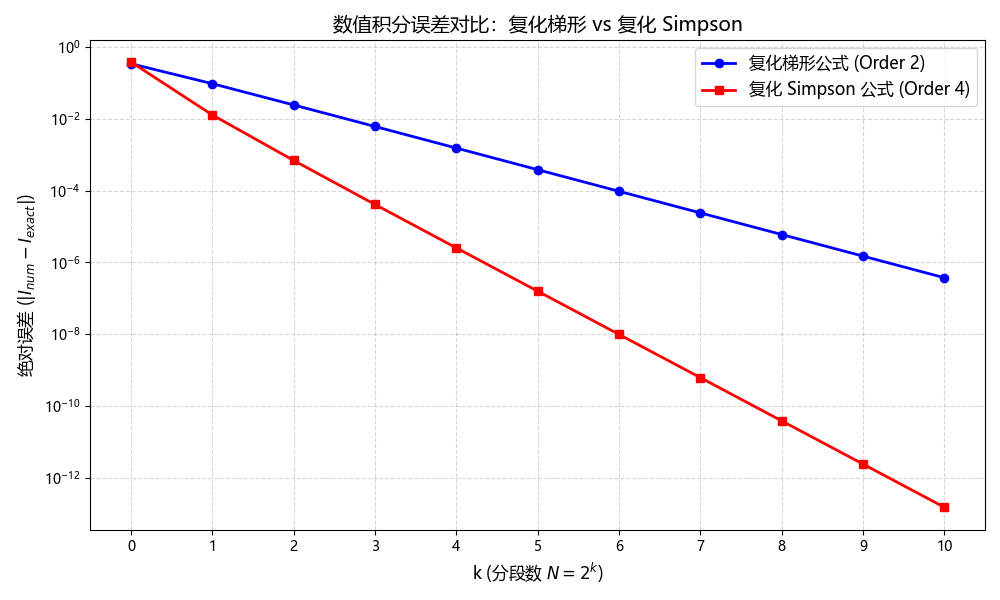
\includegraphics[width=0.8\textwidth]{plot.png}
    \caption{复化梯形与复化Simpson误差对比图}
\end{figure}
% [此处插入以 $k$ 为横坐标，$\log(|e_k|)$ 或 $e_k$ 为纵坐标的对比图像]

\section{算法分析}
本题要求实现复化 Simpson 积分公式和复化梯形积分公式的通用程序。为此，将被积函数 $f(x)$ 作为已定义函数，在两种方法中作为黑盒调用。根据题目中的公式，通过循环累加不同权重的节点函数值，分别实现了两个迭代积分算法。主函数中依次对题目要求的各分段数 $N=2^k$ 调用两种方法，并利用相邻步长的误差估算收敛阶。

实验发现，复化 Simpson 法和复化梯形法均能稳定收敛到精确解，但两者的收敛效率存在显著差异。复化梯形法表现出稳定的二阶收敛特性，误差下降曲线较缓；而复化 Simpson 法展现出极快的四阶收敛速度，在较少的节点数下（如 $N=16$）即可达到极高的精度（$10^{-6}$ 量级）。特别是在 $N=1024$ 时，Simpson 法的误差已接近计算机浮点数的机器精度极限（$10^{-13}$），体现了高阶算法的优势。

\section{实验小结}
在本次数值实验中，我分别测试了两种数值积分方法，直观地对比了误差随步长变化的趋势，验证了高阶公式在计算效率上的显著优势，同时也体会了浮点数精度对极小误差计算的影响。

复化梯形公式
\begin{itemize}
	\item 优点：几何意义明确（梯形面积逼近），算法逻辑简单，易于编程实现；对分段数 $N$ 的奇偶性无特殊要求，适用范围较广，数值稳定性好。
	\item 缺点：仅具有二阶代数精度，收敛速度较慢。为了达到较高的精度要求，往往需要将步长 $h$ 取得很小，从而大幅增加计算量。
\end{itemize}

复化 Simpson 公式
\begin{itemize}
	\item 优点：利用二次曲线拟合被积函数，在函数光滑性满足条件时具有四阶收敛速度。在相同的计算成本（节点数）下，其计算精度远高于梯形公式，效率极高。
	\item 缺点：对网格划分有一定限制（通常要求分段数 $N$ 为偶数），且计算公式中的加权系数较梯形公式略复杂；当被积函数光滑性较差时，优势可能不明显。
\end{itemize}

\end{document}